%grundlagen.tex
\chapter{Grundlagen}
\label{sec:Grundlagen}

Dieses Kapitel soll einen Überblick über die für diese Arbeit zur Verfügung stehenden Informationen sowie die darin verwendeten Tools verschaffen. Zu den Informationsquellen zählen zum einen der Datensatz der Markttransparenzstelle(MTS) für Kraftstoffe, sowie zum anderen der exemplarische Aufbau eines der auf dem Markt verfügbaren automatischen Pricing-Tools. Zusätzlich dazu liegt auch ein Erfahrungsbericht vor, wie dieses Tool bei einer Tankstelle eingesetzt wird.

\section{Datensatz}
\begin{quote} 
\glqq Seit dem 31. August 2013 sind Unternehmen, die öffentliche Tankstellen betreiben oder über die Preissetzungshoheit an diesen verfügen, verpflichtet, Preisänderungen bei den gängigen Kraftstoffsorten Super E5, Super E10 und Diesel in Echtzeit an die Markttransparenzstelle für Kraftstoffe zu melden \citep*{BkMTS}.\grqq
\end{quote}

In Echtzeit bedeutet, dass die Information über eine Preisänderung spätestens 5 Minuten nach der Änderung selber an der MTS eingehen muss. Neben den Preisänderungen müssen auch die Stammdaten der Tankstellen wöchentlich an die MTS gemeldet werden. Die MTS veröffentlicht die Daten nicht direkt selber, sondern stellt sie Verbraucherinformationsdiensten(VID) zur Verfügung. Diese verpflichten sich, die Daten in einer den Verbrauchern nützlichen Form zu veröffentlichen. Die Schnittstelle der MTS ist in der \autoref{fig:MTSK} dargestellt \citep*{IMTSK}.

\begin{figure}
	\center
	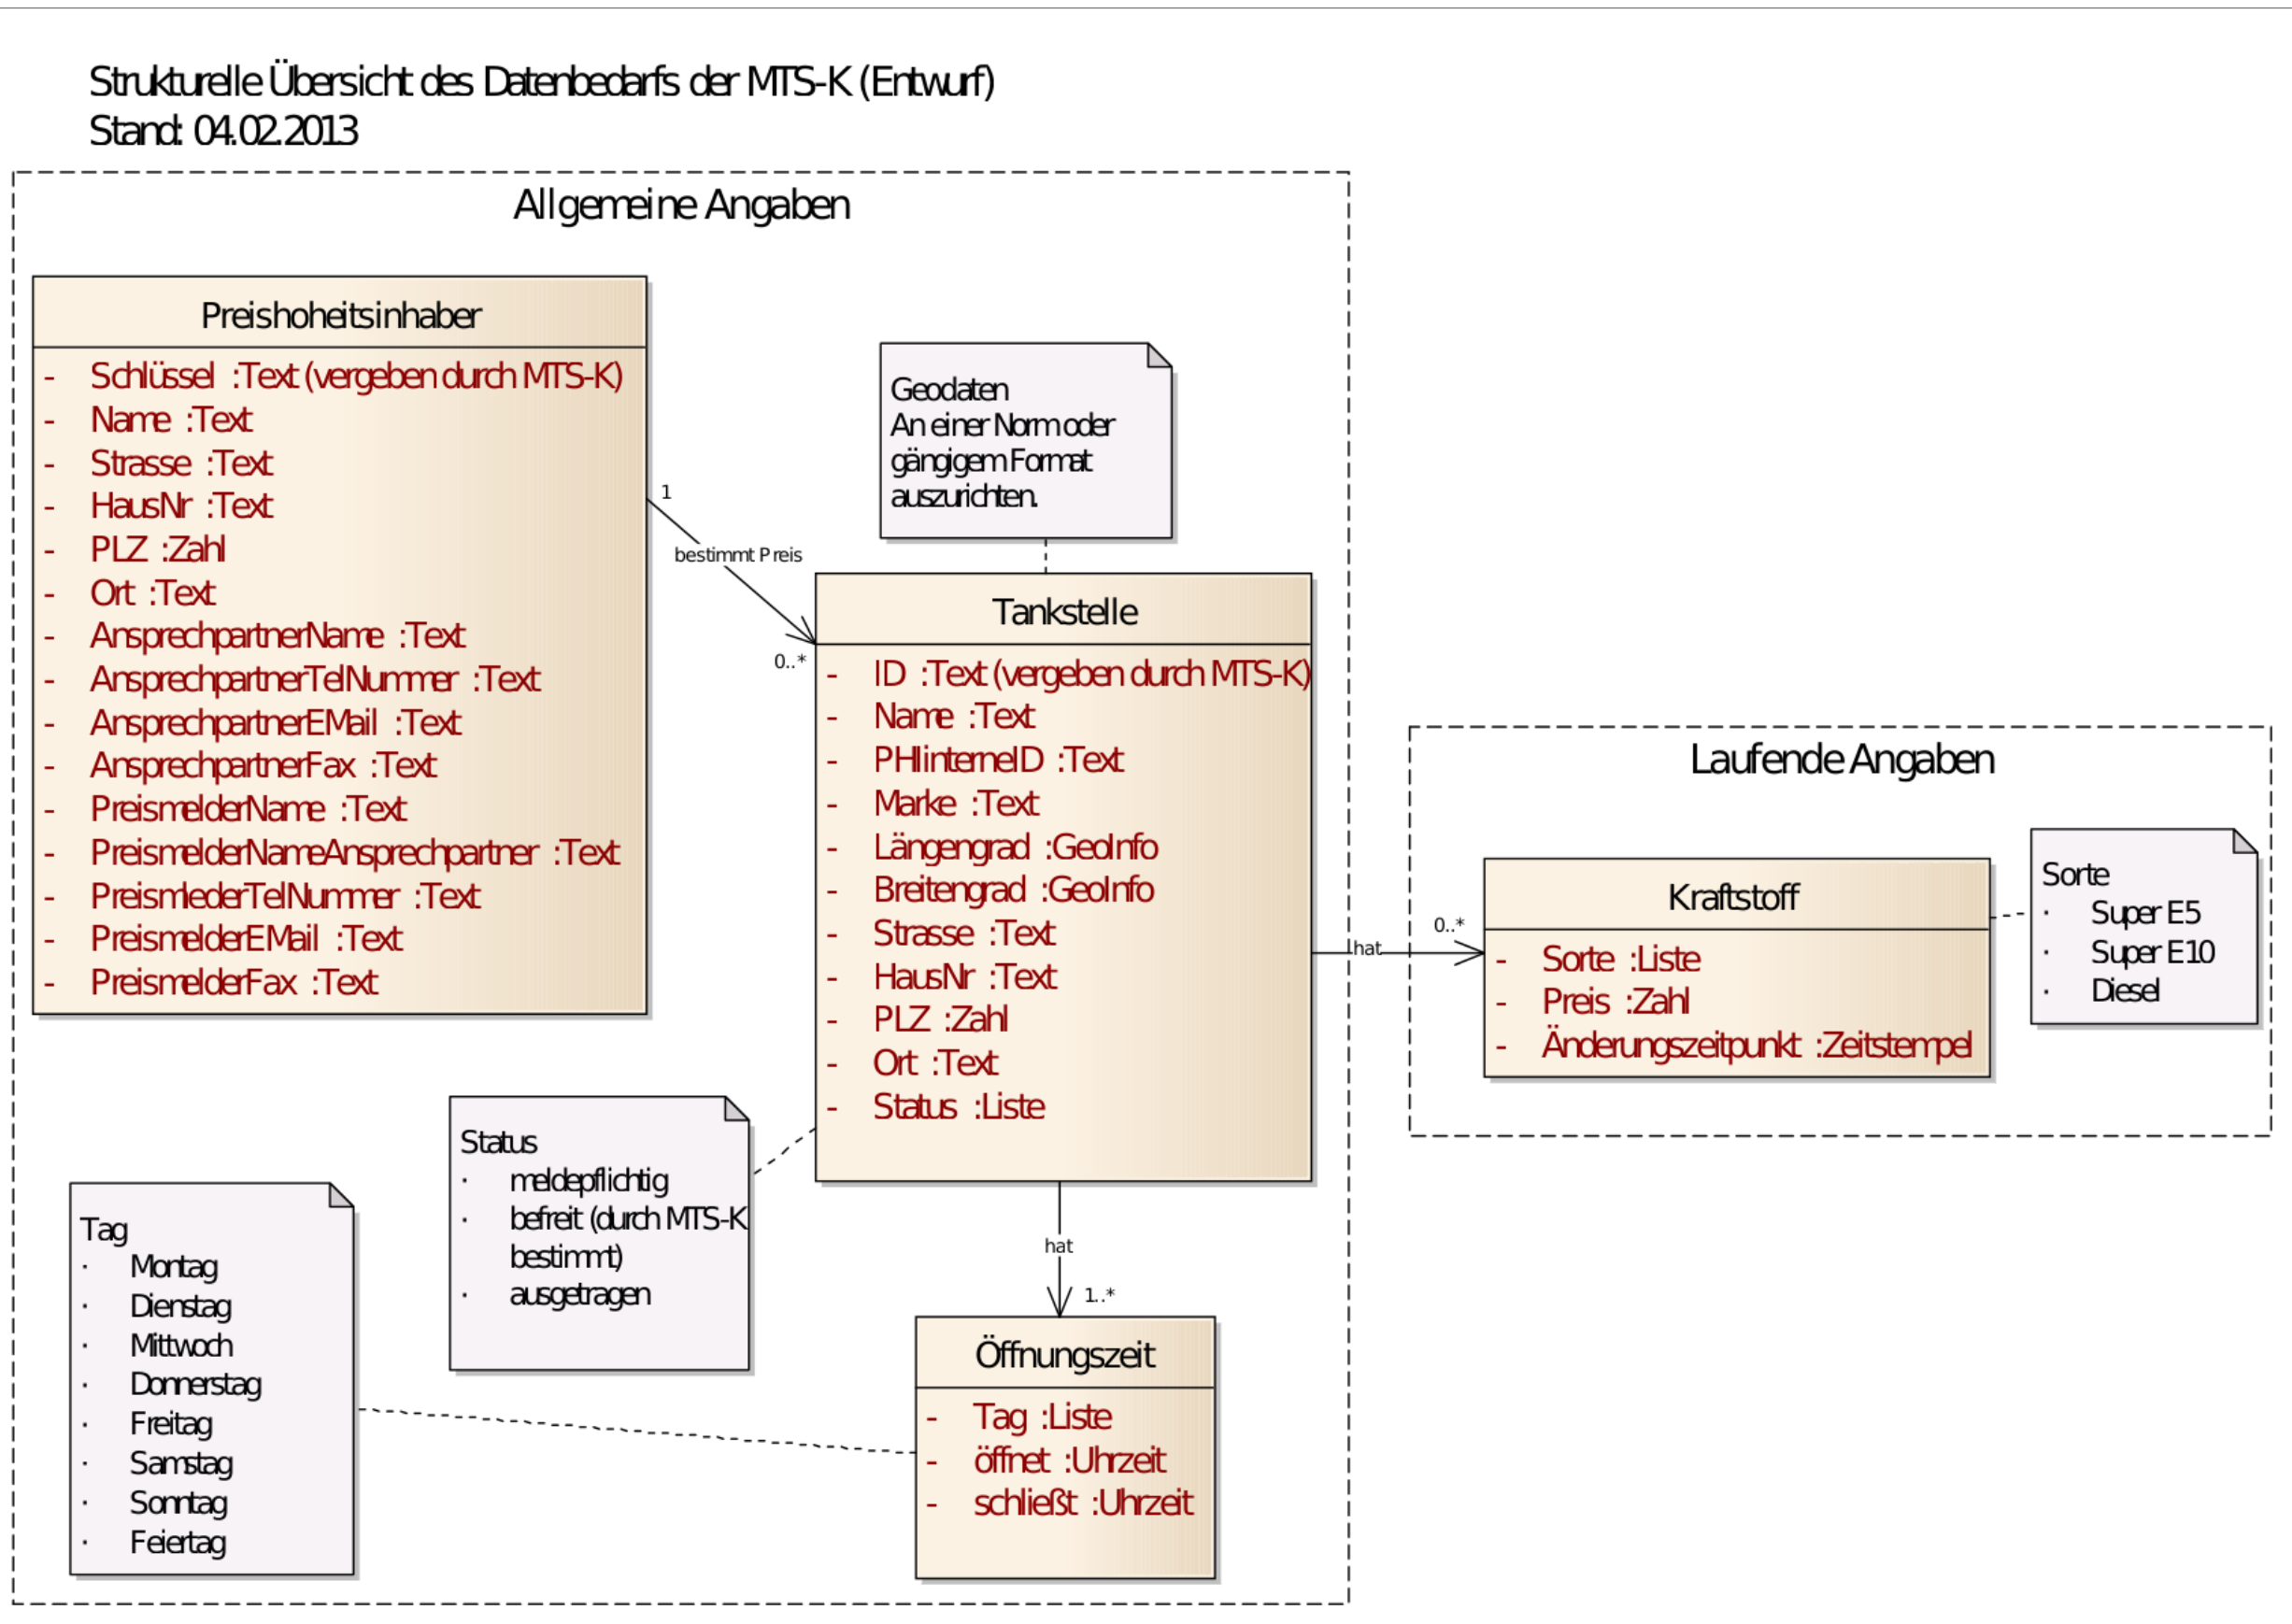
\includegraphics[width=0.8\textwidth]{Bilder/Datenstruktur-MTS.png}\\
	\caption{Datenstruktur der MTS für Kraftstoffe}
	\label{fig:MTSK}
\end{figure}

Der Datensatz für diese Arbeit entstammt dem Verbraucherinformationsdienst der \glqq Tankerkönig API \grqq. Tankerkönig bezieht seine Daten direkt von der MTS  und stellt diese sowohl im Zuge einer Echtzeit-Benzinpreis-API als auch gesondert aufbereitet als historische Datenbank in Form eines PostgreSQL-Dumps im 9.4.-Format zur Verfügung. Die für diese Arbeit verwendeten Dumps umfassen neben den kompletten Preisdaten vom 8.6.2014 bis zur aktuellsten Änderung auch die Informationen über die Stammdaten der Tankstellen \citep*{TkAPI}. 

\begin{figure}
	\center
	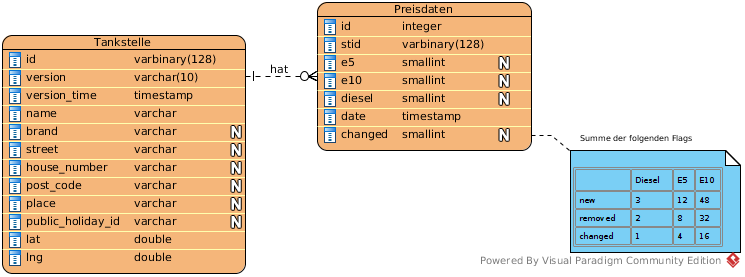
\includegraphics[width=0.8\textwidth]{Bilder/pricing_data.png}\\
	\caption{Entity-Relationship-Diagram des historischen Datensatzes}
	\label{fig:ERDT}
\end{figure}

Alle für diese Arbeit verfügbaren Informationen sind in der \autoref{fig:ERDT} abgebildet. Die Daten aus dem MTS-Datensatz werden größtenteils von den Tankstellen selber zur Verfügung gestellt, weshalb die Datenfelder teilweise nicht einheitlich definiert sind. Nur der Identifikator einer Tankstelle wird von der MTS selber bereitgestellt. Die Felder \textit{$version\_timestamp$} und \textit{version} wurden dem Datensatz von Tankerkönig hinzugefügt und geben Auskunft darüber, wann Änderungen an den Stammdaten einer Tankstelle vorgenommen wurden, beziehungsweise zählen die verschiedenen Versionen. Die Felder \textit{name} und \textit{brand} werden von den Tankstellen selber befüllt und enthalten sehr verschiedene Informationen. Bei großen Markentankstellen wird unter \textit{brand} die Marke geführt und als \textit{name} wird oft die Adresse der jeweiligen Tankstelle aufgeführt, da diese offenbar zur Identifizierung innerhalb des Unternehmens genutzt wird. Einzelne Tankstellen oder kleinere Unternehmen führen hingegen unter \textit{brand} entweder überhaupt keine Angaben oder verschiedene Bezeichnungen dafür, dass diese Tankstellen keinem größeren Konzern angehören. Bei \textit{name} geben Sie dann meistens den Inhaber oder den Unternehmensnamen an. Bei den Datenfeldern zur Adresse fehlen teilweise Informationen oder es werden Felder zusammengenommen. Beispielsweise taucht die Hausnummer des öfteren bereits im Straßenfeld mit auf. Um den Standort einer Tankstelle trotzdem eindeutig identifizieren zu können wird zusätzlich die Geolocation als Latitude and Longitude zur Verfügung gestellt. Die \textit{publi\_holiday\_id} gibt an, welchem Bundesland dieser Standort angehört um damit die entsprechend geltenden Feier- und Ferientage bestimmen zu können.\\
Bei den Preisänderungen hat Tankerkönig die neu angeschlagenen Preise der Kraftstoffsorten Diesel, E5 und E10, den Identifier der Tankstelle \textit{stid}, und den Zeitstempel \textit{date} übernommen. Zudem wurde unter \textit{id} ein Zähler über alle Änderungen, sowie mit \textit{changed} ein Kennwert für die geänderten Kraftstoffsorten hinzugefügt. Dieser Kennwert errechnet sich aus der Summe der jeweiligen Felder der kleinen Tabelle und gibt nicht nur an, ob ein Preis geändert wurde, sondern auch, ob dieser auf null gesetzt (removed), oder von Null kommend wieder erhöht (new) wurde.\\

\section{Pricing-Tool}

Neben den Verbrauchern können natürlich auch die Tankstellenbesitzer auf diese Daten zurückgreifen. Die einheitlich definierte technische Informationsschnittstelle ermöglicht es, Preise automatisch ohne Zeitverzögerung anzupassen. Zudem sind Kraftstoffe sehr homogene Güter. Homogen bedeutet, dass der Kunde das Produkt rein nach dem Preis auswählt, weil dieses an sich zwischen den Anbietern keine nennenswerten Unterschiede aufweißt. Das sorgt dafür, dass die Regeln nach denen Preise gestaltet werden eine dementsprechend einfache Struktur aufweisen können. Aus diesem Grund sind in den letzten Jahren einige Pricing-Tools enstanden, die die Preisgestaltung zumindest teilweise automatisieren. Während mittelständische Unternehmen auf externe Software Lösungen zurückgreifen, so wie zum Beispiel die Q1 und Westfalen AG auf Angebote der Firmen Temiz4u\footnotemark[1] und Weat\footnotemark[2], ist anzunehmen, dass zumindest die größten fünf Mineralölkonzerne Deutschlands (Aral, Shell, Jet, Esso und Total) intern entwickelte Programme verwenden dürften. Im Folgenden werden am Beispiel eines Tools die Einstellungsmöglichkeiten für den  Nutzer erklärt, die diesem bei der Definition seiner Regeln zur Verfügung stehen. Diese Optionen stellen gleichsam die Parameter dar, die im Zuge dieser Arbeit aus dem Datensatz extrahiert werden sollen.

\footnotetext[1]{Quelle: \url{https://www.temiz4u.net/web/guest/solutions}}
\footnotetext[2]{Quelle: \url{http://www.weat.de/produkte/pricing/}}

\subsection{Funktionsweise}
Im Folgenden werden die für diese Arbeit relevanten Funktionen eines solchen Tools beschrieben. Es wird für diese Arbeit angenommen, dass andere Tools inhaltlich ähnlich funktionieren. Das hier vorgestellte Tool erhält über einen oder mehrere Verbraucherinformationsdienste die aktuellen Preisänderungen aller Tankstellen. Beim Eintreffen einer Änderung wird überprüft, ob diese Änderung eine von dem Nutzer hinterlegte Regel verletzt. Wird eine Regel verletzt, wird darauf in der wiederum vom Nutzer gewählten Art und Weise reagiert. Die Nutzereinstellungen lassen sich in die drei Teilaspekte, \textit{Konkurrenten bestimmen, Regel festlegen und Automatisierungsgrad wählen} gliedern. 

\subsection{Konkurrenz bestimmen}
\begin{figure}[!ht]
	\center
	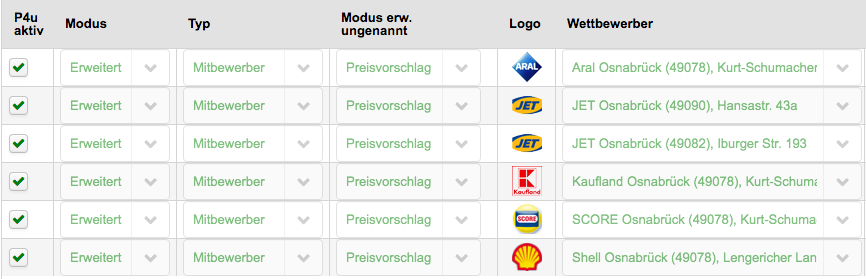
\includegraphics[width=0.8\textwidth]{Bilder/konkurenz.png}\\
	\caption{Princing Tool Einstellungsoption - Konkurrenz}
	\label{fig:PTK}
\end{figure}
Hier wird eine Liste von Tankstellen zusammengestellt, die als Konkurrenten erachtet werden. Diese Liste dient als erster Filter für die einkommenden Änderungen. Es werden im weiteren nur Änderungen überprüft, deren Tankstelle in dieser Liste vorzufinden ist.

\subsection{Regeln festlegen}
\begin{figure}[!ht]
	\center
	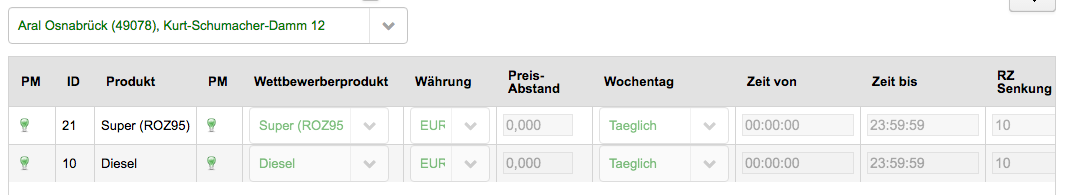
\includegraphics[width=0.8\textwidth]{Bilder/regeln1.png}\\
	\caption{Princing Tool Einstellungsoption - Regeln}
	\label{fig:PTR}
\end{figure}
Für jeden Konkurenten kann ein eigenes Regelwerk angelegt werden. Jede Regel legt zunächst einen untersten Preisabstand für eine bestimmte Spritsorte fest, welcher zu dem jeweiligen Konkurrenten gewahrt werden soll. Positive Werte besagen, dass die Tankstelle selber maximal um den genannten Betrag teuerer sein will als der entsprechende Konkurrent. Negative Werte besagen, dass die Tanstelle selber mindestens um diesen Betrag günstiger sein möchte als ihr Konkurrent. Bei dem Beispiel im Bild wären also gleiche und günstigere eigene Preise erlaubt. Zusätzlich können für den gewählten Abstand die Wochentage sowie die jeweilige Uhrzeit gewählt werden, während derer der Abstand einzuhalten ist. Wird der Abstand außerhalb dieses Zeitintervalls unterschritten, hat dies keine Konsequenzen. Im letzten Feld kann eine Reaktionszeit in Minuten angegeben werden. Diese besagt, wieviele Minuten nach dem Eingang einer regelwidrigen Änderung die gewählte Reaktion erfolgen soll.

\subsection{Automatisierung wählen}
\begin{figure}[!ht]
	\center
	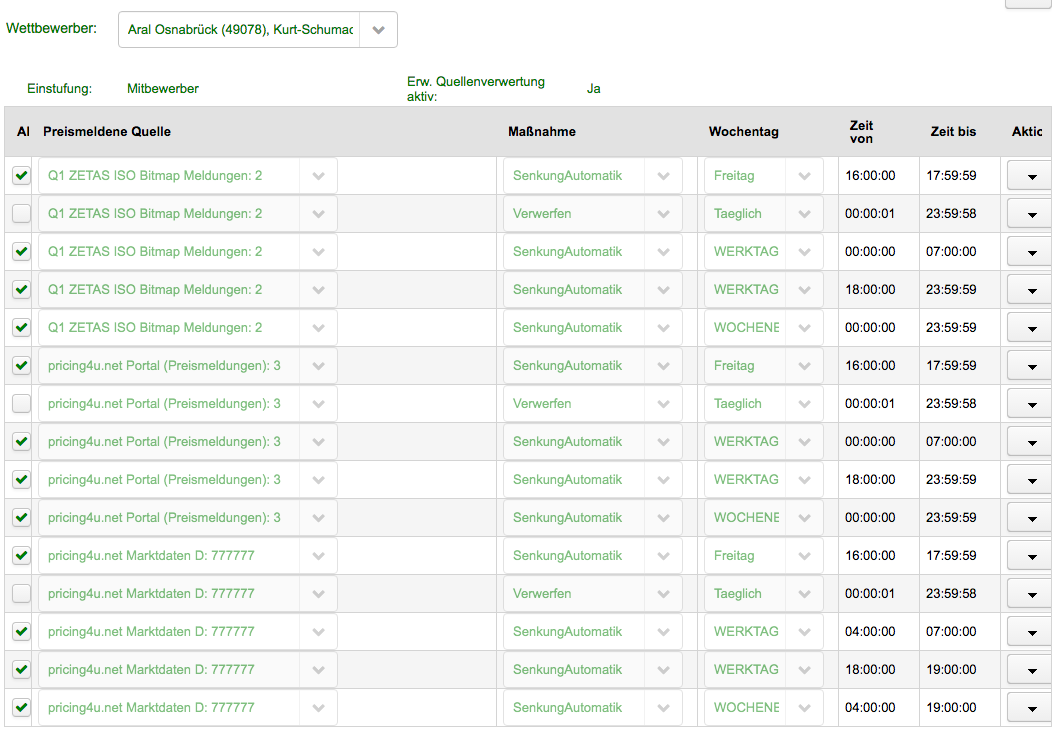
\includegraphics[width=0.8\textwidth]{Bilder/automatik.png}\\
	\caption{Princing Tool Einstellungsoption - Automatik}
	\label{fig:PTA}
\end{figure}                                                                          
Das Tool bietet neben einer \textit{default} Variante die beiden weiteren Möglichkeiten \textit{SenkungAutomatik} und \textit{Verwerfen} an, welche auf unterschiedliche Weise auf Regelverletzungen reagieren. Bei der default Variante wird bei einer Regelverletzung nach der festgelegten Reaktionszeit eine eigene Preisänderung vorgeschlagen, die den niedrigsten tolerierten Preisabstand wieder herstellt. Der Vorschlag kann dann vom Nutzer nach eigenem Ermessen durchgeführt, abgeändert oder gänzlich verworfen werden. Bei der automatischen Senkung wird anstatt eines Vorschlages die entsprechende eigene Preisänderung nach der festgelegten Reaktionszeit automatisch durchgeführt. Die letzte Möglichkeit verwirft die entsprechende Änderung ohne den Nutzer darüber zu informieren.  Wie auch schon bei den Regeln kann hier für jeden Wochentag für jedes beliebige Zeitintervall eingestellt werden, wie auf einen Verstoß reagiert werden soll.


\section{Verwendete Programme und Packages}
Das Programm zur Mustererkennung ist komplett in Python geschrieben. Es werden mit der scipy library und deren Core-Packages numpy und matplotlib die üblichen Module für den Bereich Data Mining und Machine Learning verwendet. Da die Daten als PostgreSQL-Dump zur Verfügung gestellt werden, werden sie für diese Arbeit auch wieder darin aufbereitet. Bis auf einige wenige Indexings wird von der Datenbank keinerlei Funktionalität übernommen. Indexings der Preisänderungen nach den jeweiligen Tankstellen-Ids sowie deren Zeitstempeln und der Kombination aus beiden bringt erhebliche Laufzeitverbesserungen, da die Daten hauptsächlich nach diesen Kriterien abgerufen werden. Die benötigten Daten werden mit dem PostgreSQL-Adapter psycopg aus der Datenbank geholt und dann für den kompletten Programmdurchlauf python-intern verwaltet und abgerufen. Zudem wird das Package geopy für die Berechnung des räumlichen Abstandes zwischen zwei Tankstellen anhand deren Geolocations verwendet. Die in dieser Arbeit verwendeten Visualisierungen von Barcharts, Histogrammen und anderen 2D-Graphen wurden mittels matplotlib erzeugt. Weil sich Tabellen mit diesem Tool nicht so leicht übersichtlich darstellen lassen, wurde dafür das Modul HTML.py verwendet. 